% Licensed under the Creative Commons Attribution Share Alike 4.0 International.
% See the LICENSE file in the repository root for full license text.

\section{实验:手动引用第三方库\label{sec:experiment-2}}

上一节中,我们复习了包含多个源文件的 C++ 程序的生成流程。本节我们将利用上一节的知识,探索手动引用第三方库的方法,规避可能出现的编译错误和链接错误。

\subsection*{实验步骤}

\begin{enumerate}
	\item 新建项目和源文件。操作步骤与 \ref{sec:experiment-1} 相同,项目中只包含 \lstinline[language={}]{main.cpp} 一个文件。

	\item 以源代码的形式引用 JsonCpp 库。

	JsonCpp\footnote{网址:\url{https://github.com/open-source-parsers/jsoncpp}。} 是一个用于解析 JSON 格式文本并操纵 JSON 对象的 C++ 库,而 JSON 是一种常用的数据交换格式,下面是 JSON 格式文本一例。

	\begin{lstlisting}[language={JSON}]
{
	"name": "John Doe",
	"age": 42,
	"phones": [
		{ "type": "home", "number": "555-1234" },
		{ "type": "office", "number": "555-2345" },
		{ "type": "mobile", "number": "555-3456" }
	]
}
	\end{lstlisting}

	\begin{enumerate}
		\item 下载源代码。前往 JsonCpp 最新版本的发布页面\footnote{网址:\url{https://github.com/open-source-parsers/jsoncpp/releases/tag/1.9.5}。}下载源码:\url{https://github.com/open-source-parsers/jsoncpp/archive/refs/tags/1.9.5.zip}。解压后,将其中的 \lstinline[language={}]{src} 文件夹和 \lstinline[language={}]{include} 文件夹移动到项目根目录下新建的 \lstinline[language={}]{JsonCpp} 文件夹中。

		\item 将源文件添加到项目中。在 Dev-C++ 中打开新建的项目,在“项目管理”窗口中右键点击项目,点击弹出菜单中的“添加文件夹”,命名为“JsonCpp”。在“项目管理”窗口中右键点击刚才新建的“JsonCpp”文件夹,点击弹出菜单中的“添加”,进入项目目录下的 \lstinline[language={}]{JsonCpp/src/lib_json},选择其中所有以 \lstinline[language={}]{.cpp} 为扩展名的文件,点击“打开”。完成后的“项目管理”窗口如图 \ref{fig:manual-library-1} 所示。

		\begin{figure}
			\centering
			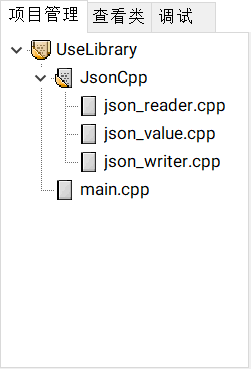
\includegraphics[width=0.2\linewidth]{assets/manual-library-1}
			\caption{添加源文件后的“项目管理”窗口。}
			\label{fig:manual-library-1}
		\end{figure}

		\item 将包含目录添加到项目中。在“项目管理”窗口中右键点击项目,点击弹出菜单中的“项目属性”。在弹出的对话框中,点击“文件/目录”选项卡,再点击“包含文件目录”子选项卡。点击右下角的选择文件夹按钮(图 \ref{fig:manual-library-2} 中的蓝色按钮),选择项目目录下的 \lstinline[language={}]{JsonCpp/include} 文件夹,按钮旁的编辑框将显示完整路径。删除其中的绝对路径,只保留 \lstinline[language={}]{JsonCpp/include},然后点击“添加”。完成后的“项目属性”对话框如图 \ref{fig:manual-library-3} 所示\footnote{也可以直接在编辑框中输入 \lstinline[language={}]{JsonCpp/include},不点击选择文件夹按钮。}。最后点击“确定”退出该对话框。

		\begin{figure}
			\centering
			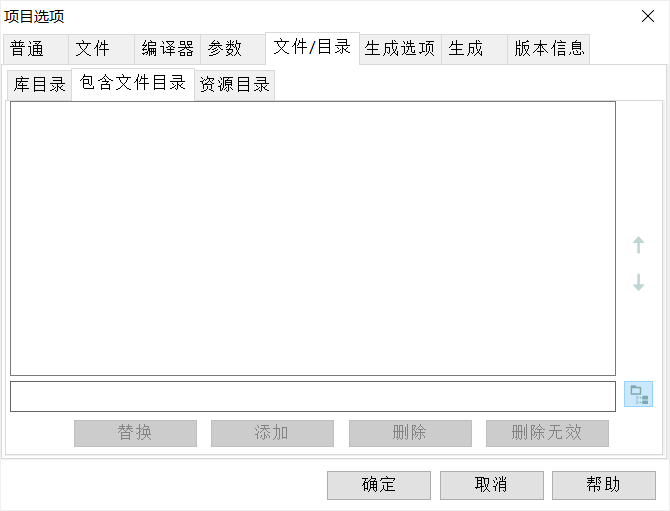
\includegraphics[width=0.75\linewidth]{assets/manual-library-2}
			\caption{“项目属性”对话框。}
			\label{fig:manual-library-2}
		\end{figure}

		\begin{figure}
			\centering
			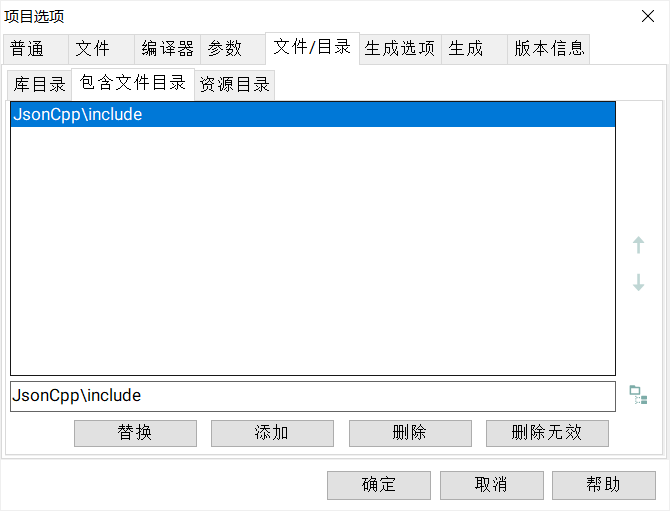
\includegraphics[width=0.75\linewidth]{assets/manual-library-3}
			\caption{完成后的“项目属性”对话框。}
			\label{fig:manual-library-3}
		\end{figure}

		\item 编写代码。

		\begin{lstlisting}[language={[17]C++}, moreemph={[1]Value}]
// main.cpp
#include <json/json.h>

int main()
{
	Json::Value v = 1;
}
	\end{lstlisting}

		\item 编译并运行代码。“编译日志”窗口记录的命令如下。

		\begin{lstlisting}[language={}]
g++.exe -c main.cpp -o main.o -I"C:/Program Files (x86)/Embarcadero/Dev-Cpp/TDM-GCC-64/include" -I"JsonCpp/include"

g++.exe -c JsonCpp/src/lib_json/json_reader.cpp -o JsonCpp/src/lib_json/json_reader.o -I"C:/Program Files (x86)/Embarcadero/Dev-Cpp/TDM-GCC-64/include" -I"JsonCpp/include"

g++.exe -c JsonCpp/src/lib_json/json_value.cpp -o JsonCpp/src/lib_json/json_value.o -I"C:/Program Files (x86)/Embarcadero/Dev-Cpp/TDM-GCC-64/include" -I"JsonCpp/include"

g++.exe -c JsonCpp/src/lib_json/json_writer.cpp -o JsonCpp/src/lib_json/json_writer.o -I"C:/Program Files (x86)/Embarcadero/Dev-Cpp/TDM-GCC-64/include" -I"JsonCpp/include"

g++.exe main.o JsonCpp/src/lib_json/json_reader.o JsonCpp/src/lib_json/json_value.o JsonCpp/src/lib_json/json_writer.o -o UseLibrary.exe -L"C:/Program Files (x86)/Embarcadero/Dev-Cpp/TDM-GCC-64/lib" -static-libgcc
		\end{lstlisting}
	\end{enumerate}

	\item 以二进制的形式引用 SFML 库。

	SFML\footnote{网址:\url{https://www.sfml-dev.org/}。} 全称 Simple and Fast Multimedia Library,是一个用于编写游戏和多媒体应用程序的多媒体库。一般而言,多媒体库较为复杂,从源码构建需要较长的时间,所以下面我们将以二进制的形式引用 SFML 库。

	\begin{enumerate}
		\item 下载源代码和二进制文件。前往 SFML 的代码仓库\footnote{网址:\url{https://github.com/SFML/SFML}。},在最新版本的发布页面\footnote{网址:\url{https://github.com/SFML/SFML/releases/tag/2.5.1}。}下载发布的文件:\url{https://github.com/SFML/SFML/releases/download/2.5.1/SFML-2.5.1-windows-gcc-7.3.0-mingw-64-bit.zip}。注意,此处要选择与你使用的编译器相匹配的版本。将整个 \lstinline[language={}]{SFML-2.5.1} 文件解压到项目根目录下。

		\item 将包含目录添加到项目中。操作步骤与此前相同,添加的包含目录为 \lstinline[language={}]{SFML-2.5.1/include}。完成后的“项目属性”对话框如图 \ref{fig:manual-library-4} 所示。

		\begin{figure}
			\centering
			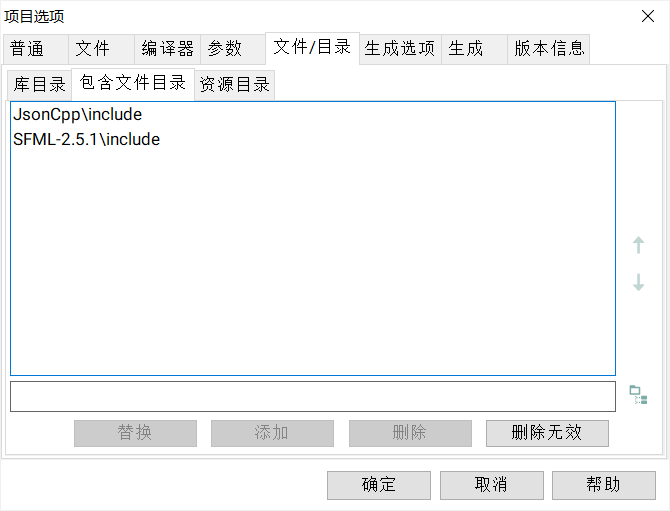
\includegraphics[width=0.75\linewidth]{assets/manual-library-4}
			\caption{添加包含目录后的“项目属性”对话框。}
			\label{fig:manual-library-4}
		\end{figure}

		\item 将附加链接库添加到项目中。在“项目属性”对话框中,进入“参数”选项卡,点击“链接”文本框下的“加入库或者对象”,选择项目目录下 \lstinline[language={}]{SFML-2.5.1/lib} 中所有扩展名为 \lstinline[language={}]{.a} 的文件。完成后的“项目属性”对话框如图 \ref{fig:manual-library-5} 所示。

		\begin{figure}
			\centering
			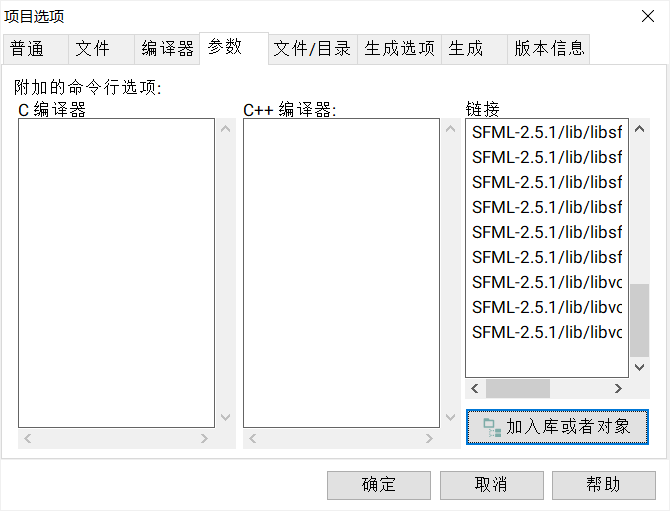
\includegraphics[width=0.75\linewidth]{assets/manual-library-5}
			\caption{添加附加链接库后的“项目属性”对话框。}
			\label{fig:manual-library-5}
		\end{figure}

		\item 编写代码。

		\begin{lstlisting}[language={[17]C++}, moreemph={[1]Value, Window, VideoMode, Event}, moreemph={[2]isOpen, pollEvent, close, display}]
// main.cpp
#include <json/json.h>
#include <SFML/Window.hpp>

int main()
{
    Json::Value v = 1;
    sf::Window window(sf::VideoMode(640, 480), "Hello, world!");
    while (window.isOpen())
    {
        sf::Event event;
        while (window.pollEvent(event))
        {
            if (event.type == sf::Event::Closed)
                window.close();
        }
        window.display();
    }
}
		\end{lstlisting}

		\item 编译代码。“编译日志”窗口记录的命令如下(第 3 行的命令是节选)。

		\begin{lstlisting}[language={}]
g++.exe -c main.cpp -o main.o -I"C:/Program Files (x86)/Embarcadero/Dev-Cpp/TDM-GCC-64/include" -I"JsonCpp/include" -I"SFML-2.5.1/include"

g++.exe main.o JsonCpp/src/lib_json/json_reader.o JsonCpp/src/lib_json/json_value.o JsonCpp/src/lib_json/json_writer.o -o UseLibrary.exe -L"C:/Program Files (x86)/Embarcadero/Dev-Cpp/TDM-GCC-64/lib" -static-libgcc SFML-2.5.1/lib/libFLAC.a SFML-2.5.1/lib/libfreetype.a ...
		\end{lstlisting}

		\item 将动态链接库拷贝到可执行文件所在目录。将 \lstinline[language={}]{SFML/bin} 中所有的 \lstinline[language={}]{.dll} 文件拷贝到项目根目录中,保证生成的 \lstinline[language={}]{.exe} 文件与这些 \lstinline[language={}]{.dll} 文件位于同一目录,如图 \ref{fig:manual-library-6} 所示。

		\begin{figure}
			\centering
			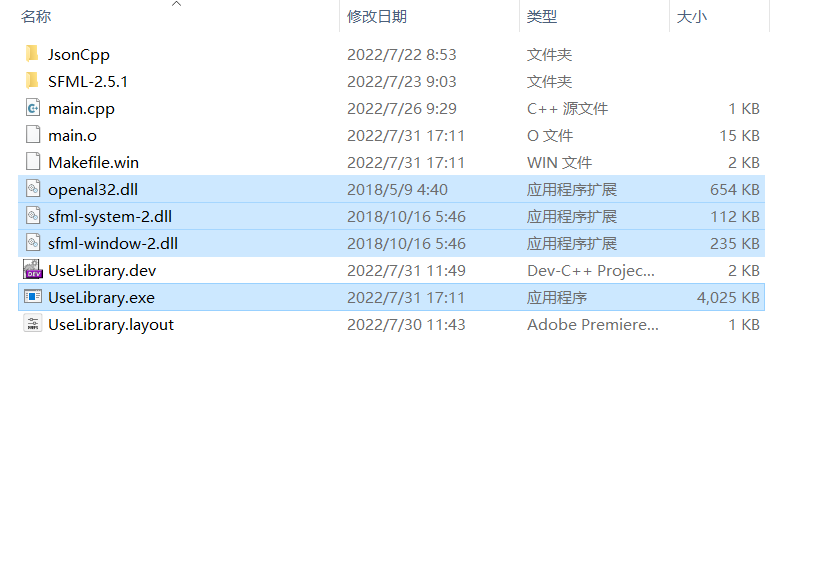
\includegraphics[width=0.75\linewidth]{assets/manual-library-6}
			\caption{需要保证所有 \lstinline[language={}]{.dll} 文件与 \lstinline[language={}]{.exe} 文件位于同一目录。}
			\label{fig:manual-library-6}
		\end{figure}

		\item 运行程序。在 Dev-C++ 中点击菜单栏中的“运行”、“运行”,可以看到一个控制台窗口和一个黑色窗口弹出,如图 \ref{fig:manual-library-7} 所示。

		\begin{figure}
			\centering
			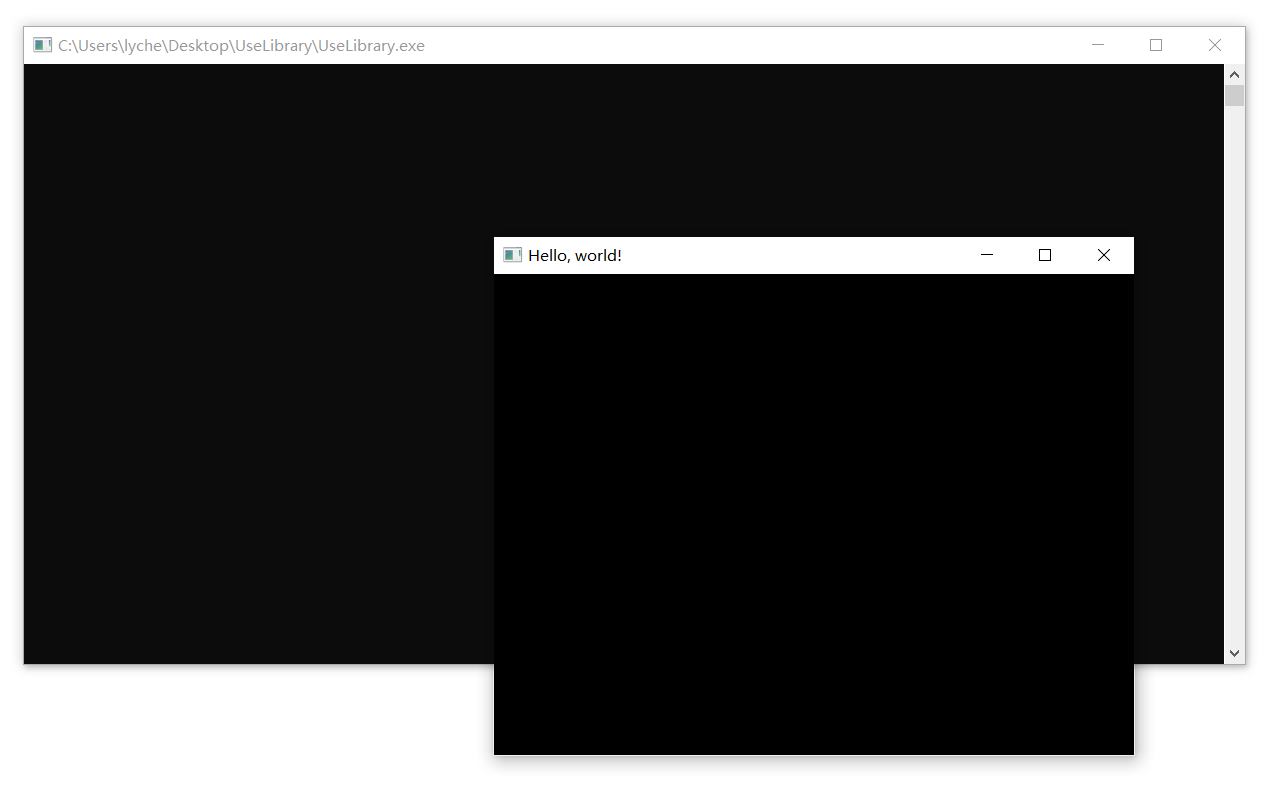
\includegraphics[width=0.75\linewidth]{assets/manual-library-7}
			\caption{程序运行结果。}
			\label{fig:manual-library-7}
		\end{figure}
	\end{enumerate}
\end{enumerate}
